\chapter{Target Architecture and Solution Design (To-Be)}
\label{chap:architecture}

This chapter presents the target architecture resulting from the decision framework in Chapter~\ref{chap:methodology}. The baseline is described in Chapter~\ref{chap:baseline}; here the focus is on the migration destination designed for incremental adoption.

\section{Architecture Overview}
The migration of Outsight Cloud to AWS required a cloud-native architecture able to improve scalability, maintainability, and service integration while preserving the original application workflow. The selected design follows a layered model with four levels: a client and delivery layer, a load balancing and routing layer, an application layer, and a managed services layer. The resulting left-to-right request flow starts from the browser, continues through CloudFront and an Application Load Balancer, reaches frontend and backend services on ECS Fargate, and integrates with managed services including PostgreSQL, Redis, Amazon S3, Cognito, SES, and SNS (Figure~\ref{fig:outsight-to-be-architecture}).

\begin{figure}[htbp]
    \centering
    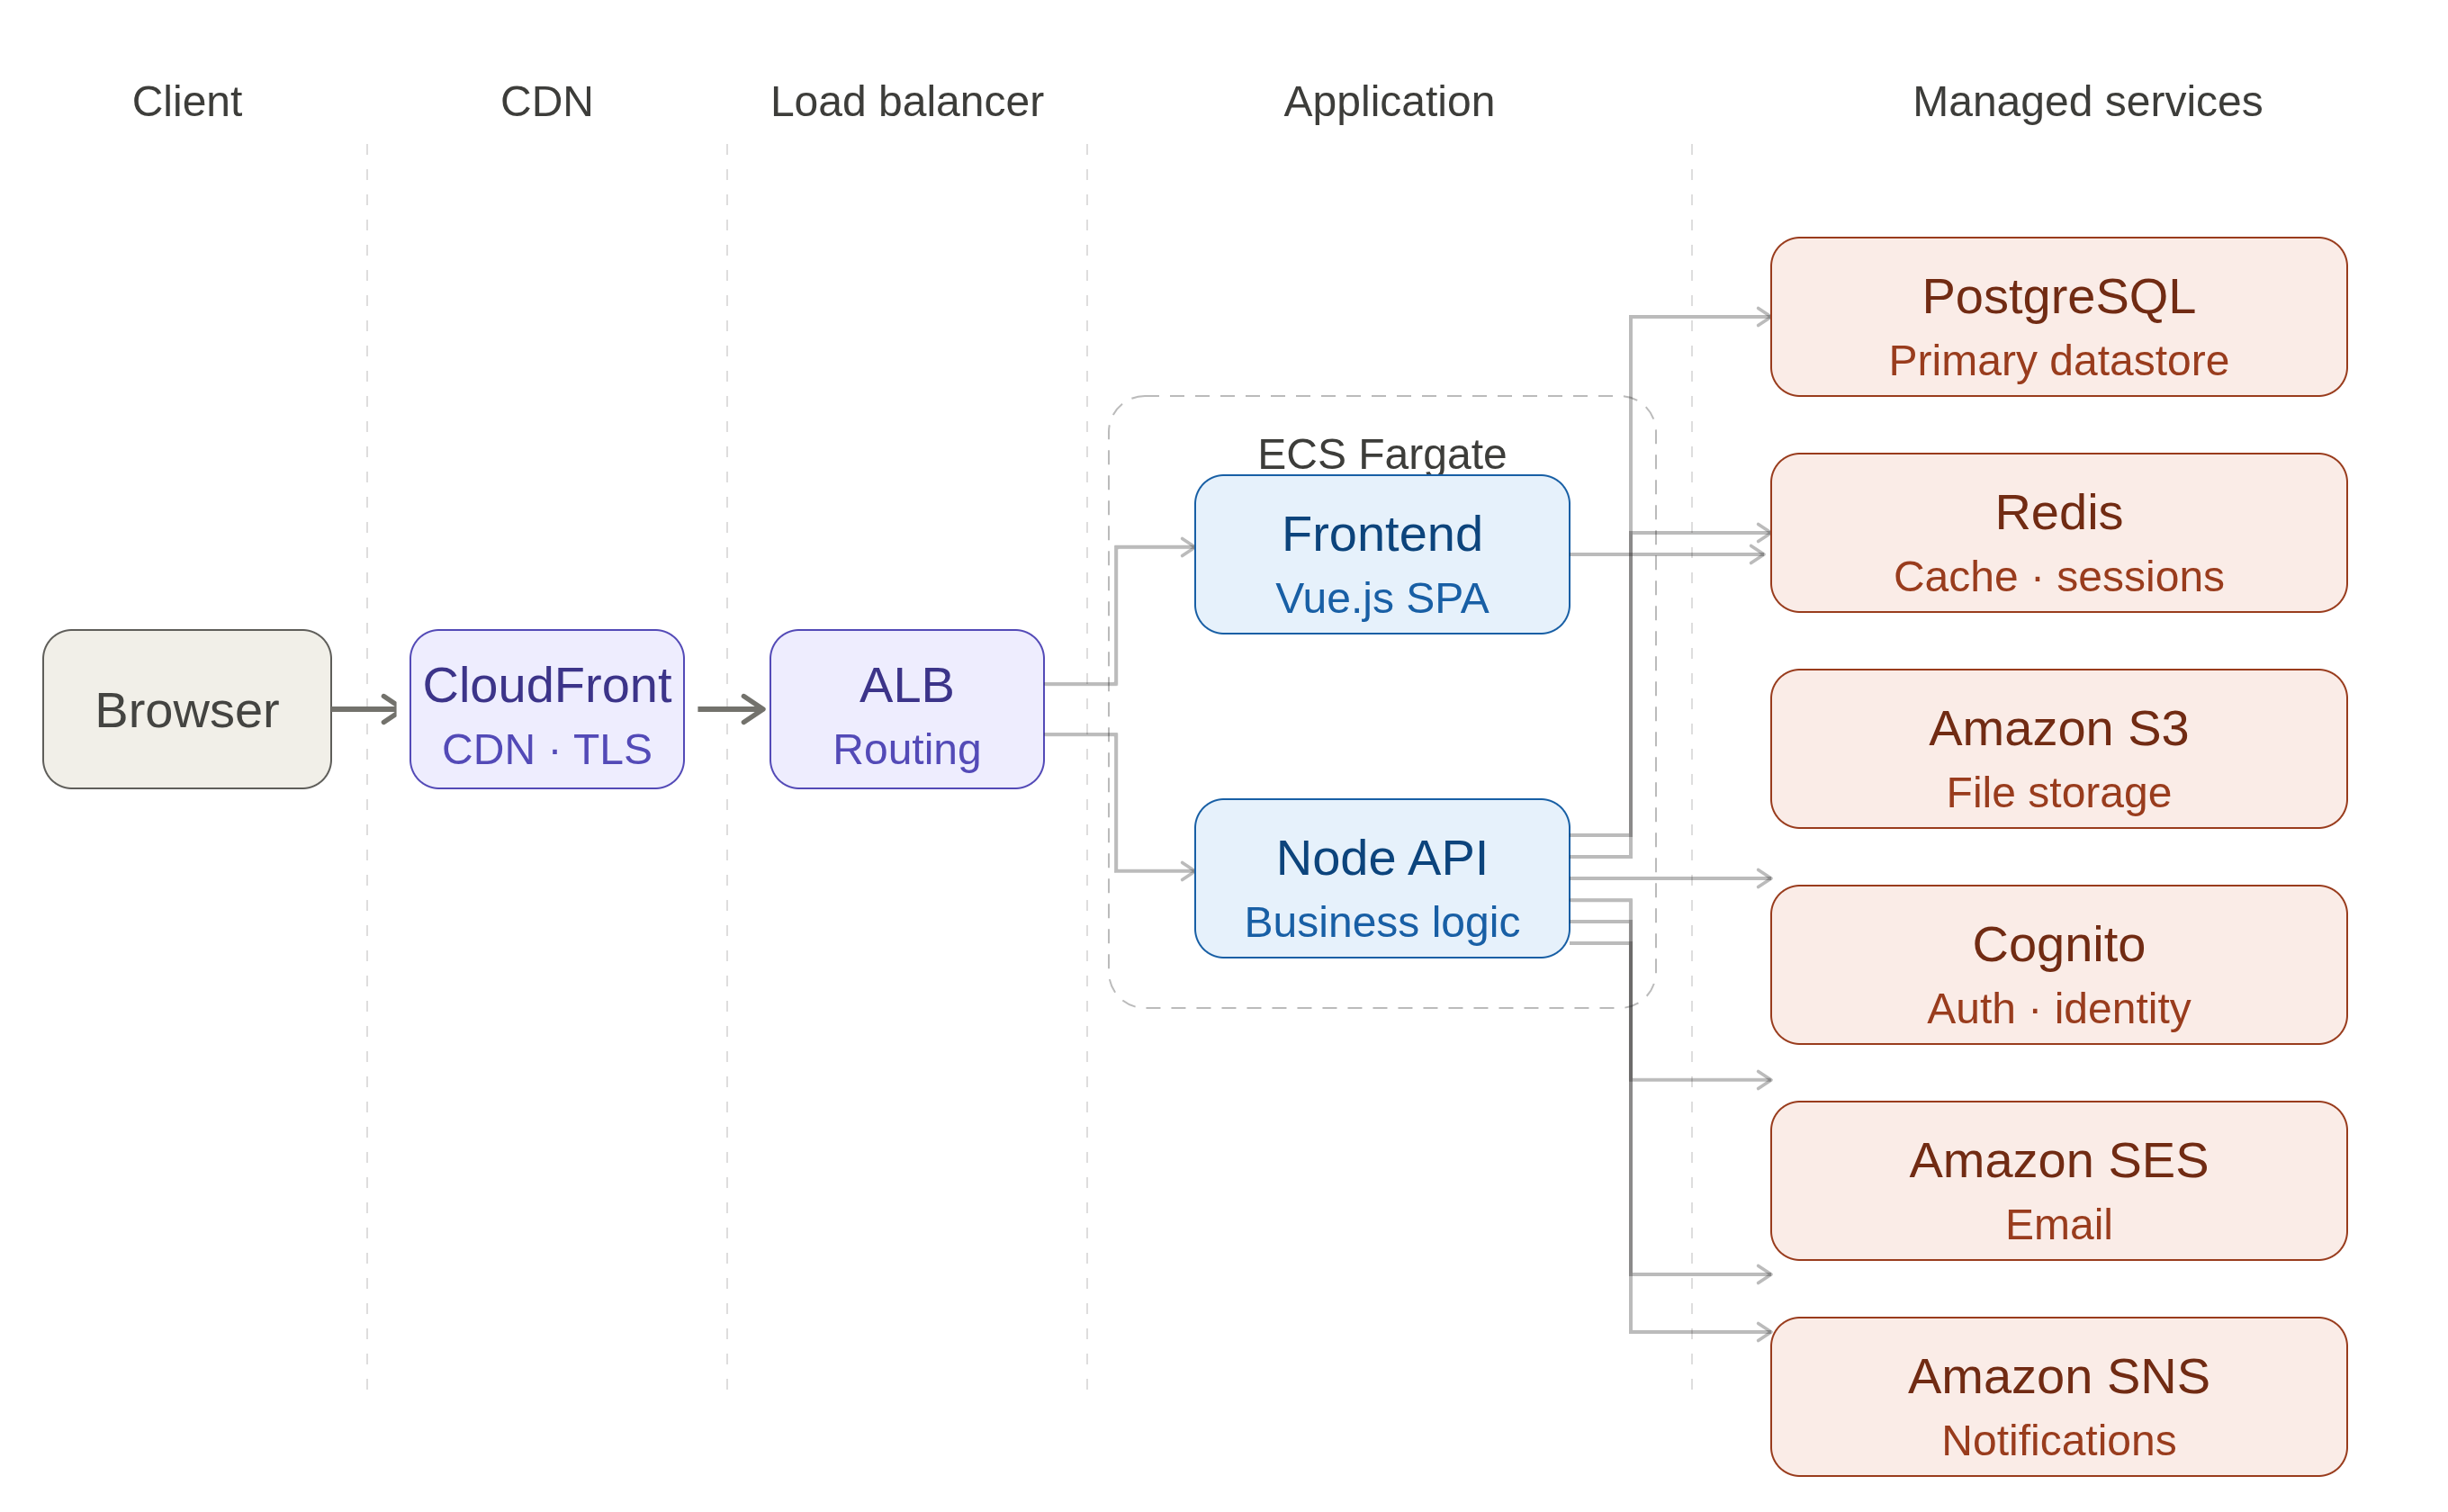
\includegraphics[width=0.95\textwidth]{immagini/outsight_aws_architecture.png}
    \caption{Final AWS architecture adopted for Outsight Cloud.}
    \label{fig:outsight-to-be-architecture}
\end{figure}

\section{Client, Delivery, and Routing Layers}
The browser is the user entry point to Outsight Cloud, used for simulation visualization, organization and site management, document access, and file operations, all over HTTPS. \textbf{Amazon CloudFront} acts as the content delivery layer between users and the internal infrastructure, reducing latency, caching static assets, and reducing backend load, which is particularly relevant for the Vue frontend static resources. The \textbf{Application Load Balancer} (ALB) is the central routing component: it receives requests forwarded by CloudFront and distributes traffic across ECS Fargate services, providing request routing, health checks, HTTPS termination, and traffic distribution, enabling independent scaling and improved fault tolerance.

\section{Application Layer}
The application layer runs on \textbf{Amazon ECS Fargate} with a serverless container execution model that removes the need to provision, patch, and scale virtual machines manually. This choice follows the evaluation in Chapter~\ref{chap:methodology}: Kubernetes was not selected because the associated cluster-management overhead was not justified by the scale of Outsight Cloud during the migration. The \textbf{frontend service} (Vue.js) renders the user interface, handles interactions, and manages authentication flows, while the \textbf{backend service} (Node.js) exposes the core APIs orchestrating business logic for organizations, sites, simulations, authentication, file operations, notifications, and integrations with AWS services. Deploying each as a dedicated container enables independent release and scaling.

\section{Managed Services Layer}
\textbf{PostgreSQL} replaced Airtable as primary data storage, moving from a semi-structured backend toward a relational model with stronger consistency guarantees; core entities such as users, organizations, sites, and simulations are persisted there. \textbf{Redis} is used as in-memory cache and session storage to reduce persistent-storage accesses and improve response time. \textbf{Amazon S3} provides object storage for simulation files, uploaded assets, and documentation, selected for scalability, durability, and native AWS integration. \textbf{Amazon Cognito} handles authentication and identity management (registration, login, verification, token handling), reducing custom authentication logic. \textbf{Amazon SES} handles outgoing email (invitations, account messages, notifications), and \textbf{Amazon SNS} supports asynchronous, event-driven notifications for decoupled communication patterns.

\section{Network and Security Topology}
The AWS deployment was designed around a simplified cloud-native networking model focused on incremental migration and controlled exposure of public services. The infrastructure operates inside an AWS Virtual Private Cloud (VPC) with multiple public subnets across Availability Zones to improve availability. ECS Fargate services run with public outbound connectivity to simplify communication with managed services and reduce networking overhead during early stages. Despite the use of public subnets, direct external access to containers is restricted through dedicated Security Groups: the ALB accepts inbound HTTP/HTTPS traffic from external clients, ECS services accept traffic only from the ALB, and containers are therefore not directly exposed to the Internet. TLS is managed through AWS Certificate Manager (ACM) for centralized certificate lifecycle management. The architecture also separates application traffic from static asset delivery: simulation files are stored in private S3 buckets distributed through CloudFront, with access restricted through CloudFront Origin Access Control (OAC). Overall, the topology reflects a pragmatic migration-oriented design balancing security and operational simplicity while preserving the possibility of future evolution toward more isolated network architectures.

\section{Architectural Benefits}
Compared to the legacy architecture of Chapter~\ref{chap:baseline}, the target design directly addresses the migration drivers of Chapter~\ref{chap:intro} and the decision criteria of Chapter~\ref{chap:methodology}. First, it provides clearer separation of concerns between presentation, application services, data storage, and supporting services, reducing coupling and simplifying future evolution. Second, the adoption of managed services significantly reduces operational responsibility, delegating load balancing, TLS management, storage scalability, and database availability to AWS. Third, it improves scalability: frontend and backend scale independently through ECS Fargate, and managed storage and database services evolve independently from application deployments. From a maintainability standpoint, Infrastructure as Code through Terraform establishes a reproducible, version-controlled infrastructure model, reducing configuration drift. The migration from Airtable to PostgreSQL further strengthens ownership of the data layer through explicit relational schemas and database-level constraints. Finally, environment separation, automated provisioning, and the validation mechanisms described in Chapter~\ref{chap:implementation} provide a stronger foundation for controlled deployments and incremental evolution. Overall, the final AWS architecture is not simply a replacement hosting environment but a cloud-native operational model designed for long-term sustainability.
